\documentclass[11pt,letterpaper]{article}

% ============================================================================
% PACKAGES
% ============================================================================
\usepackage[utf8]{inputenc}
\usepackage[T1]{fontenc}
\usepackage{helvet}
\renewcommand{\familydefault}{\sfdefault}
\usepackage[margin=0.85in, headheight=28pt]{geometry}
\usepackage{graphicx}
\usepackage{xcolor}
\usepackage{tikz}
\usepackage{tcolorbox}
\usepackage{booktabs}
\usepackage{enumitem}
\usepackage{hyperref}
\usepackage{fancyhdr}
\usepackage{titlesec}
\usepackage{multicol}
\usepackage{listings}
\usepackage{upquote}
\usepackage{amsmath,amssymb}
\usepackage{pgfplots}
\usepackage{array}
\usepackage{longtable}
\usepackage{colortbl}
\usepackage{pifont}
\usepackage{setspace}
\usepackage{parskip}
\usepackage{caption}

\pgfplotsset{compat=1.18}
\usetikzlibrary{shapes.geometric, arrows.meta, positioning, calc, decorations.pathreplacing, backgrounds, fit, shadows.blur, matrix, patterns, fadings, shadings}

% ============================================================================
% COLOR DEFINITIONS - Modern AWS/Cloud Palette
% ============================================================================
\definecolor{awsdark}{HTML}{161E2D}         % Deep navy
\definecolor{awsblue}{HTML}{232F3E}         % AWS dark blue
\definecolor{awsorange}{HTML}{FF9900}       % AWS signature orange
\definecolor{awslightorange}{HTML}{FFAC33}  % Lighter orange
\definecolor{cloudblue}{HTML}{4A90D9}       % Sky blue
\definecolor{cloudlight}{HTML}{E8F4FD}      % Light cloud
\definecolor{successgreen}{HTML}{2ECC71}    % Success green
\definecolor{warningamber}{HTML}{F39C12}    % Warning amber
\definecolor{dangerred}{HTML}{E74C3C}       % Danger red
\definecolor{infoteal}{HTML}{17A2B8}        % Info teal
\definecolor{coolgray}{HTML}{6C757D}        % Cool gray
\definecolor{lightgray}{HTML}{F8F9FA}       % Light background
\definecolor{codebg}{HTML}{2D2D2D}          % Dark code background
\definecolor{codetext}{HTML}{F8F8F2}        % Light code text

% ============================================================================
% HYPERREF SETUP
% ============================================================================
\hypersetup{
  colorlinks=true,
  linkcolor=cloudblue,
  urlcolor=awsorange,
  pdftitle={AWS Bedrock AgentCore Memory Integration Guide},
  pdfauthor={AI Agent Team}
}

% ============================================================================
% SPACING AND TYPOGRAPHY
% ============================================================================
\setstretch{1.15}
\setlength{\parskip}{0.5em}
\setlist{nosep, leftmargin=1.5em, itemsep=0.3em}

% ============================================================================
% PAGE STYLE
% ============================================================================
\pagestyle{fancy}
\fancyhf{}
\fancyhead[L]{%
  \begin{tikzpicture}[baseline=-0.5ex]
    \fill[awsorange] (0,0) circle (0.15);
    \fill[awsorange!70] (0.35,0) circle (0.1);
    \fill[awsorange!40] (0.6,0) circle (0.06);
  \end{tikzpicture}
  \hspace{0.3em}\textcolor{awsblue}{\textsf{\textbf{AgentCore Memory}}}%
}
\fancyhead[R]{\textcolor{coolgray}{\textsf{\thepage}}}
\fancyfoot[C]{\textcolor{coolgray}{\small\textsf{AWS Bedrock AgentCore Integration Guide}}}
\renewcommand{\headrulewidth}{0pt}
\renewcommand{\footrulewidth}{0pt}

% Add subtle top border
\fancyheadoffset{0pt}
\setlength{\headheight}{32pt}

% ============================================================================
% SECTION FORMATTING - Modern Style
% ============================================================================
\titleformat{\section}
  {\normalfont\LARGE\bfseries\color{awsblue}}
  {\colorbox{awsorange}{\textcolor{white}{\thesection}}}{0.8em}{}
\titleformat{\subsection}
  {\normalfont\Large\bfseries\color{awsblue!80}}
  {\thesubsection}{0.6em}{}
\titleformat{\subsubsection}
  {\normalfont\large\color{coolgray}\bfseries}
  {\thesubsubsection}{0.5em}{}

\titlespacing*{\section}{0pt}{3ex plus 1ex minus .2ex}{2ex plus .2ex}
\titlespacing*{\subsection}{0pt}{2.5ex plus 1ex minus .2ex}{1.5ex plus .2ex}

% ============================================================================
% TOC STYLING
% ============================================================================
\setcounter{tocdepth}{2}

% ============================================================================
% TCOLORBOX ENVIRONMENTS - Modern Redesign
% ============================================================================
\tcbuselibrary{skins,breakable,hooks}

% Key Concept Box - Gradient left border
\newtcolorbox{keybox}[1][Key Concept]{
  enhanced,
  breakable,
  colback=cloudlight,
  colframe=cloudblue,
  colbacktitle=cloudblue,
  coltitle=white,
  fonttitle=\bfseries\sffamily,
  title={\faLightbulb\hspace{0.5em}#1},
  boxrule=0pt,
  leftrule=4pt,
  arc=0pt,
  outer arc=0pt,
  left=12pt, right=12pt, top=8pt, bottom=8pt,
  shadow={2pt}{-2pt}{0pt}{black!20}
}

% Warning Box - Bold left accent
\newtcolorbox{warnbox}[1][Warning]{
  enhanced,
  breakable,
  colback=dangerred!5,
  colframe=dangerred,
  colbacktitle=dangerred,
  coltitle=white,
  fonttitle=\bfseries\sffamily,
  title={\faExclamationTriangle\hspace{0.5em}#1},
  boxrule=0pt,
  leftrule=4pt,
  arc=0pt,
  outer arc=0pt,
  left=12pt, right=12pt, top=8pt, bottom=8pt,
  shadow={2pt}{-2pt}{0pt}{black!15}
}

% Success/Tip Box
\newtcolorbox{tipbox}[1][Pro Tip]{
  enhanced,
  breakable,
  colback=successgreen!8,
  colframe=successgreen,
  colbacktitle=successgreen,
  coltitle=white,
  fonttitle=\bfseries\sffamily,
  title={\faCheckCircle\hspace{0.5em}#1},
  boxrule=0pt,
  leftrule=4pt,
  arc=0pt,
  outer arc=0pt,
  left=12pt, right=12pt, top=8pt, bottom=8pt,
  shadow={2pt}{-2pt}{0pt}{black!15}
}

% AWS Service Box - Orange accent
\newtcolorbox{awsbox}[1][AWS Service]{
  enhanced,
  breakable,
  colback=awsorange!5,
  colframe=awsorange,
  colbacktitle=awsorange,
  coltitle=white,
  fonttitle=\bfseries\sffamily,
  title={\faAws\hspace{0.5em}#1},
  boxrule=0pt,
  leftrule=4pt,
  arc=0pt,
  outer arc=0pt,
  left=12pt, right=12pt, top=8pt, bottom=8pt,
  shadow={2pt}{-2pt}{0pt}{black!15}
}

% Info Box - Teal accent
\newtcolorbox{infobox}[1][Note]{
  enhanced,
  breakable,
  colback=infoteal!5,
  colframe=infoteal,
  colbacktitle=infoteal,
  coltitle=white,
  fonttitle=\bfseries\sffamily,
  title={\faInfoCircle\hspace{0.5em}#1},
  boxrule=0pt,
  leftrule=4pt,
  arc=0pt,
  outer arc=0pt,
  left=12pt, right=12pt, top=8pt, bottom=8pt,
  shadow={2pt}{-2pt}{0pt}{black!15}
}

% TL;DR Summary Box - Prominent
\newtcolorbox{tldrbox}{
  enhanced,
  breakable,
  colback=awsblue!3,
  colframe=awsblue,
  boxrule=1.5pt,
  arc=8pt,
  outer arc=8pt,
  left=15pt, right=15pt, top=12pt, bottom=12pt,
  fontupper=\small,
  before upper={\textcolor{awsorange}{\faRocket}\hspace{0.5em}\textbf{TL;DR}\hspace{0.8em}},
  shadow={3pt}{-3pt}{0pt}{black!20}
}

% ============================================================================
% CODE LISTING STYLE - Dark Theme with Enhanced Captions
% ============================================================================
\lstdefinestyle{moderncode}{
  language=Python,
  basicstyle=\ttfamily\small\color{codetext},
  keywordstyle=\color{cloudblue}\bfseries,
  stringstyle=\color{successgreen},
  commentstyle=\color{coolgray}\itshape,
  backgroundcolor=\color{codebg},
  frame=none,
  numbers=left,
  numberstyle=\tiny\color{coolgray},
  numbersep=10pt,
  breaklines=true,
  showstringspaces=false,
  tabsize=4,
  xleftmargin=20pt,
  framexleftmargin=15pt,
  aboveskip=1.5em,
  belowskip=1em,
  literate={`}{\`}1
}
\lstset{style=moderncode}

% Custom caption format for listings
\DeclareCaptionFormat{codecaption}{%
  \begin{tcolorbox}[
    enhanced,
    colback=awsblue!5,
    colframe=awsblue!50,
    boxrule=0.5pt,
    arc=4pt,
    left=8pt, right=8pt, top=4pt, bottom=4pt,
    before skip=0pt,
    after skip=0.5em
  ]
  \textcolor{awsblue}{\faFileCode}\hspace{0.5em}\small\sffamily #1#2#3
  \end{tcolorbox}
}
\captionsetup[lstlisting]{format=codecaption, labelfont={bf}, textfont={}, skip=0pt}

% ============================================================================
% ICON COMMANDS (pifont replacements for fontawesome5)
% ============================================================================
\newcommand{\faRobot}{\ding{70}}
\newcommand{\faCheck}{\ding{51}}
\newcommand{\faCheckCircle}{\ding{51}}
\newcommand{\faTimes}{\ding{55}}
\newcommand{\faTimesCircle}{\ding{55}}
\newcommand{\faExclamationTriangle}{\ding{74}}
\newcommand{\faExclamationCircle}{\ding{74}}
\newcommand{\faLightbulb}{\ding{72}}
\newcommand{\faInfoCircle}{\ding{73}}
\newcommand{\faRocket}{\ding{228}}
\newcommand{\faDatabase}{\ding{115}}
\newcommand{\faTachometerAlt}{\ding{99}}
\newcommand{\faAws}{\textbf{AWS}}
\newcommand{\faCloud}{\ding{110}}
\newcommand{\faBrain}{\ding{70}}
\newcommand{\faServer}{\ding{115}}
\newcommand{\faProjectDiagram}{\ding{118}}
\newcommand{\faLayerGroup}{\ding{115}}
\newcommand{\faCode}{\texttt{</>}}
\newcommand{\faCogs}{\ding{70}}
\newcommand{\faShieldAlt}{\ding{110}}
\newcommand{\faKey}{\ding{70}}
\newcommand{\faEye}{\ding{70}}
\newcommand{\faCloudUploadAlt}{\ding{110}}
\newcommand{\faChartLine}{\ding{70}}
\newcommand{\faDollarSign}{\$}
\newcommand{\faBook}{\ding{70}}
\newcommand{\faFileCode}{\ding{70}}
\newcommand{\faPython}{\ding{70}}
\newcommand{\faGithub}{\ding{70}}
\newcommand{\faListAlt}{\ding{70}}
\newcommand{\faClock}{\ding{70}}
\newcommand{\faSearch}{\ding{70}}
\newcommand{\faCalculator}{\ding{70}}
\newcommand{\faBan}{\ding{55}}
\newcommand{\faFileAlt}{\ding{70}}
\newcommand{\faRandom}{\ding{70}}
\newcommand{\faEraser}{\ding{70}}
\newcommand{\faLock}{\ding{70}}
\newcommand{\faUserShield}{\ding{70}}

% ============================================================================
% CUSTOM COMMANDS
% ============================================================================
\newcommand{\api}[1]{\texttt{\textcolor{cloudblue}{#1}}}
\newcommand{\code}[1]{\texttt{\small\colorbox{lightgray}{#1}}}
\newcommand{\ratelimit}{\textcolor{dangerred}{\faExclamationCircle\ 0.25 req/sec}}

% ============================================================================
% PART PAGE STYLING
% ============================================================================
\newcommand{\partpage}[4]{%
  \clearpage
  \thispagestyle{empty}
  \begin{tikzpicture}[remember picture, overlay]
    % Gradient background
    \shade[top color=awsdark, bottom color=awsblue]
      (current page.north west) rectangle ([yshift=-9cm]current page.north east);

    % Decorative circles
    \fill[awsorange, opacity=0.15] ([xshift=12cm, yshift=-3cm]current page.north west) circle (4cm);
    \fill[awsorange, opacity=0.1] ([xshift=14cm, yshift=-6cm]current page.north west) circle (2.5cm);
    \fill[cloudblue, opacity=0.1] ([xshift=3cm, yshift=-5cm]current page.north west) circle (3cm);

    % Part number - large and prominent
    \node[white, opacity=0.08, font=\fontsize{200}{200}\selectfont\bfseries]
      at ([xshift=5cm, yshift=-5cm]current page.north west) {#1};

    % Part label
    \node[white, font=\large\sffamily] at ([yshift=-2.5cm]current page.north) {PART};

    % Part number (visible)
    \node[awsorange, font=\fontsize{72}{72}\selectfont\bfseries]
      at ([yshift=-4.5cm]current page.north) {#1};

    % Part title
    \node[white, font=\Huge\bfseries\sffamily] at ([yshift=-7cm]current page.north) {#2};

    % Decorative line
    \draw[awsorange, line width=2pt]
      ([xshift=5cm, yshift=-8cm]current page.north west) --
      ([xshift=-5cm, yshift=-8cm]current page.north east);
  \end{tikzpicture}

  \vspace{9.5cm}

  % Overview content
  \begin{center}
  \begin{minipage}{0.88\textwidth}
    \begin{tcolorbox}[
      enhanced,
      colback=white,
      colframe=awsorange!50,
      boxrule=1pt,
      arc=6pt,
      left=15pt, right=15pt, top=12pt, bottom=12pt,
      shadow={2pt}{-2pt}{0pt}{black!15}
    ]
    \textcolor{awsblue}{\faListAlt\hspace{0.5em}\textbf{What's Covered}}
    \vspace{0.5em}

    #3
    \end{tcolorbox}

    \vspace{1em}

    % Icon row
    \begin{center}
    #4
    \end{center}
  \end{minipage}
  \end{center}
}

% ============================================================================
% DOCUMENT
% ============================================================================
\begin{document}

% ============================================================================
% TITLE PAGE - Modern Redesign
% ============================================================================
\begin{titlepage}

\begin{tikzpicture}[remember picture, overlay]
  % Main gradient background
  \shade[left color=awsdark, right color=awsblue!90]
    (current page.north west) rectangle ([xshift=8cm]current page.south west);

  % Decorative elements on left panel
  \foreach \y/\s/\o in {-4/1.2/0.1, -8/0.8/0.08, -12/1.5/0.06, -18/1/0.12, -22/0.6/0.08} {
    \fill[awsorange, opacity=\o] ([xshift=4cm, yshift=\y cm]current page.north west) circle (\s cm);
  }

  % Enhanced Memory network visualization on left
  \begin{scope}[shift={([xshift=4cm, yshift=-14cm]current page.north west)}]
    % Outer glow ring
    \foreach \r/\o in {3/0.03, 2.7/0.05, 2.4/0.07} {
      \fill[awsorange, opacity=\o] (0,0) circle (\r);
    }

    % Central hub with gradient effect
    \shade[ball color=awsorange] (0,0) circle (0.7);
    \node[white, font=\small\bfseries] at (0,0) {MEM};

    % Agent nodes with connecting pulses
    \foreach \angle/\label/\col in {72/C/cloudblue, 144/G/successgreen, 216/O/infoteal, 288/X/warningamber, 0/R/dangerred} {
      % Connection line with gradient
      \draw[white, opacity=0.5, line width=2pt, dashed] (0,0) -- (\angle:1.8);
      % Node outer glow
      \fill[\col, opacity=0.2] (\angle:2.3) circle (0.55);
      % Node
      \fill[\col, opacity=0.8] (\angle:2.3) circle (0.4);
      \node[white, font=\scriptsize\bfseries] at (\angle:2.3) {\label};
      % Data packet traveling on line
      \fill[white] (\angle:1.2) circle (0.1);
    }

    % Inner orbiting data ring
    \foreach \i in {1,...,16} {
      \fill[white, opacity={0.3+0.3*rand}] ({22.5*\i}:1.1) circle (0.06);
    }

    % Outer knowledge particles
    \foreach \i in {1,...,8} {
      \fill[awsorange, opacity=0.6] ({45*\i + 20}:2.9) circle (0.08);
    }
  \end{scope}

  % Right side content area background
  \fill[white] ([xshift=8cm]current page.north west) rectangle (current page.south east);

  % Subtle grid pattern on white area
  \foreach \x in {9,10,...,20} {
    \draw[lightgray, opacity=0.3] ([xshift=\x cm]current page.north west) -- ([xshift=\x cm]current page.south west);
  }
  \foreach \y in {-2,-4,...,-26} {
    \draw[lightgray, opacity=0.3] ([xshift=8cm, yshift=\y cm]current page.north west) -- ([yshift=\y cm]current page.north east);
  }
\end{tikzpicture}

% Title content
\begin{tikzpicture}[remember picture, overlay]
  % AWS badge
  \node[fill=awsorange, rounded corners=3pt, inner sep=6pt] at ([xshift=12cm, yshift=-3cm]current page.north west) {
    \textcolor{white}{\small\bfseries\sffamily AWS BEDROCK}
  };

  % Main title
  \node[anchor=west, text width=11cm] at ([xshift=9cm, yshift=-6cm]current page.north west) {
    {\fontsize{48}{52}\selectfont\bfseries\color{awsblue}AgentCore}\\[0.3cm]
    {\fontsize{36}{40}\selectfont\color{cloudblue}Memory}\\[0.2cm]
    {\Large\color{coolgray}\sffamily Integration Guide}
  };

  % Tagline
  \node[anchor=west] at ([xshift=9cm, yshift=-10.5cm]current page.north west) {
    \textcolor{awsblue}{\large\sffamily Persistent Memory for AI Agent Ecosystems}
  };

  % Divider line
  \draw[awsorange, line width=3pt]
    ([xshift=9cm, yshift=-11.5cm]current page.north west) --
    ([xshift=19cm, yshift=-11.5cm]current page.north west);

  % Description
  \node[anchor=north west, text width=10cm] at ([xshift=9cm, yshift=-12.5cm]current page.north west) {
    \color{coolgray}\normalsize
    Enable your AI agents to remember context across sessions, share knowledge,
    and leverage semantic search---all backed by AWS managed infrastructure.
  };

  % Key metrics row
  \node[anchor=north west] at ([xshift=9cm, yshift=-16cm]current page.north west) {
    \begin{tikzpicture}
      % Metric 1
      \node[fill=lightgray, rounded corners=8pt, minimum width=3.2cm, minimum height=2.2cm] (m1) at (0,0) {};
      \node[awsorange, font=\Large] at ([yshift=0.4cm]m1.center) {\faDatabase};
      \node[awsblue, font=\LARGE\bfseries] at (m1.center) {3};
      \node[coolgray, font=\scriptsize] at ([yshift=-0.5cm]m1.center) {Memory Providers};

      % Metric 2
      \node[fill=lightgray, rounded corners=8pt, minimum width=3.2cm, minimum height=2.2cm] (m2) at (4,0) {};
      \node[dangerred, font=\Large] at ([yshift=0.4cm]m2.center) {\faTachometerAlt};
      \node[awsblue, font=\LARGE\bfseries] at (m2.center) {0.25};
      \node[coolgray, font=\scriptsize] at ([yshift=-0.5cm]m2.center) {req/sec (events)};

      % Metric 3
      \node[fill=lightgray, rounded corners=8pt, minimum width=3.2cm, minimum height=2.2cm] (m3) at (8,0) {};
      \node[successgreen, font=\Large] at ([yshift=0.4cm]m3.center) {\faRobot};
      \node[awsblue, font=\LARGE\bfseries] at (m3.center) {5+};
      \node[coolgray, font=\scriptsize] at ([yshift=-0.5cm]m3.center) {AI Agents};
    \end{tikzpicture}
  };

  % Part navigation
  \node[anchor=north west] at ([xshift=9cm, yshift=-20cm]current page.north west) {
    \begin{tikzpicture}
      \foreach \i/\label/\col in {1/Architecture/awsblue, 2/Implementation/awsblue!80, 3/Security/awsblue!60, 4/Operations/awsblue!40} {
        \node[fill=\col, text=white, rounded corners=4pt, minimum width=2.4cm, minimum height=0.9cm, font=\small\bfseries] at ({(\i-1)*2.7},0) {Part \i};
        \node[coolgray, font=\scriptsize] at ({(\i-1)*2.7},-0.8) {\label};
      }
    \end{tikzpicture}
  };

  % Memory flow diagram at bottom
  \node[anchor=north] at ([xshift=14cm, yshift=-23cm]current page.north west) {
    \begin{tikzpicture}[
      membox/.style={rectangle, rounded corners=6pt, minimum width=3.5cm, minimum height=1.4cm, font=\small\sffamily},
      arrow/.style={->, thick, >=stealth}
    ]
      \node[membox, fill=infoteal!15, draw=infoteal] (short) at (0,0) {
        \textbf{Short-Term}\\[-2pt]
        \tiny Session Events
      };
      \node[membox, fill=successgreen!15, draw=successgreen] (long) at (5.5,0) {
        \textbf{Long-Term}\\[-2pt]
        \tiny Persistent Facts
      };

      \draw[arrow, awsorange, line width=1.5pt] (short) -- node[above, font=\tiny, color=coolgray] {extraction} (long);

      \node[dangerred, font=\tiny] at ([yshift=-0.9cm]short.south) {\faExclamationCircle\ Rate Limited};
      \node[successgreen, font=\tiny] at ([yshift=-0.9cm]long.south) {\faCheckCircle\ No Limit};
    \end{tikzpicture}
  };

  % Version footer
  \node[anchor=south, coolgray, font=\footnotesize\sffamily] at ([yshift=1.5cm]current page.south) {
    Version 1.0 \textbar\ \today
  };
\end{tikzpicture}
\end{titlepage}

% ============================================================================
% EXECUTIVE SUMMARY
% ============================================================================
\newpage
\thispagestyle{empty}

\begin{center}
{\color{awsblue}\fontsize{28}{32}\selectfont\bfseries Executive Summary}
\end{center}

\vspace{1cm}

\begin{tldrbox}
AI agents are stateless. This integration adds persistent memory via AWS Bedrock AgentCore,
enabling cross-session context and shared knowledge across your entire agent ecosystem.
\end{tldrbox}

\vspace{1.5em}

% Enhanced Problem/Solution/Constraint cards with side icons
\begin{tikzpicture}
  \node[fill=dangerred!8, rounded corners=10pt, text width=0.88\textwidth, inner sep=15pt, anchor=north west,
        drop shadow={shadow xshift=2pt, shadow yshift=-2pt, opacity=0.15}] (prob) at (1.2,0) {
    \textcolor{dangerred}{\textbf{THE PROBLEM}}\\[0.5em]
    \color{awsblue}AI agents (Claude Code, Gemini, OpenCode, Crush, Codex) lose all context between sessions.
    Each conversation starts from scratch---no memory of codebase patterns, user preferences, or prior learnings.
  };
  % Side icon
  \node[fill=dangerred, circle, minimum size=1cm, inner sep=0pt] at (0.4, -0.7) {
    \textcolor{white}{\large\faBrain}
  };
\end{tikzpicture}

\vspace{0.8em}

\begin{tikzpicture}
  \node[fill=successgreen!8, rounded corners=10pt, text width=0.88\textwidth, inner sep=15pt, anchor=north west,
        drop shadow={shadow xshift=2pt, shadow yshift=-2pt, opacity=0.15}] at (1.2,0) {
    \textcolor{successgreen}{\textbf{THE SOLUTION}}\\[0.5em]
    \color{awsblue}AWS Bedrock AgentCore Memory provides managed short-term and long-term memory.
    A new MCP server bridges your local agents with cloud-based persistent storage.
  };
  % Side icon
  \node[fill=successgreen, circle, minimum size=1cm, inner sep=0pt] at (0.4, -0.7) {
    \textcolor{white}{\large\faCloud}
  };
\end{tikzpicture}

\vspace{0.8em}

\begin{tikzpicture}
  \node[fill=awsorange!8, rounded corners=10pt, text width=0.88\textwidth, inner sep=15pt, anchor=north west,
        drop shadow={shadow xshift=2pt, shadow yshift=-2pt, opacity=0.15}] at (1.2,0) {
    \textcolor{awsorange}{\textbf{KEY CONSTRAINT}}\\[0.5em]
    \color{awsblue}The \api{CreateEvent} API is rate-limited to \textbf{0.25 req/sec per actor+session}.
    This is NOT a logging system---use it for sparse, high-value events only.
    Long-term facts via \api{BatchCreateMemoryRecords} have no such limit.
  };
  % Side icon
  \node[fill=awsorange, circle, minimum size=1cm, inner sep=0pt] at (0.4, -0.7) {
    \textcolor{white}{\large\faTachometerAlt}
  };
\end{tikzpicture}

\vspace{1.5em}

% API Overview Table
\begin{center}
\renewcommand{\arraystretch}{1.4}
\begin{tabular}{>{\raggedright}p{3.5cm} >{\centering}p{5cm} >{\raggedright\arraybackslash}p{5.5cm}}
\rowcolor{awsblue!10}
\textbf{\color{awsblue}Memory Type} & \textbf{\color{awsblue}API} & \textbf{\color{awsblue}Use Case} \\
\midrule
Short-term events & \api{CreateEvent} \textcolor{dangerred}{\tiny(0.25/s)} & Session goals, key decisions \\
Long-term facts & \api{BatchCreateMemoryRecords} & Patterns, preferences, learnings \\
Semantic search & \api{RetrieveMemoryRecords} & Context retrieval by meaning \\
\bottomrule
\end{tabular}
\end{center}

\vspace{2em}

% Architecture Preview
\begin{center}
\begin{tikzpicture}[
  layer/.style={rectangle, rounded corners=6pt, minimum height=1.2cm, font=\small\sffamily},
  arrow/.style={->, thick, >=stealth, awsblue!70}
]
  % Agents layer
  \node[layer, fill=cloudlight, draw=cloudblue, minimum width=12cm] (agents) at (0,2) {
    \faRobot\ \ Claude \quad\faRobot\ \ Gemini \quad\faRobot\ \ OpenCode \quad\faRobot\ \ Crush \quad\faRobot\ \ Codex
  };

  % MCP layer
  \node[layer, fill=awsblue!10, draw=awsblue, minimum width=12cm] (mcp) at (0,0) {
    \textbf{mcp-agentcore-memory} \textcolor{coolgray}{(aiobotocore)}
  };

  % AWS layer
  \node[layer, fill=awsorange!10, draw=awsorange, minimum width=12cm] (aws) at (0,-2) {
    \faAws\ \ AWS Bedrock AgentCore Memory
  };

  \draw[arrow] (agents) -- (mcp);
  \draw[arrow, awsorange] (mcp) -- node[right, font=\tiny, color=coolgray] {HTTPS} (aws);

  % Labels
  \node[coolgray, font=\tiny, anchor=east] at ([xshift=-0.5cm]agents.west) {Self-Hosted};
  \node[coolgray, font=\tiny, anchor=east] at ([xshift=-0.5cm]aws.west) {AWS Cloud};
\end{tikzpicture}
\end{center}

% ============================================================================
% TABLE OF CONTENTS
% ============================================================================
\newpage
\tableofcontents
\newpage

% ============================================================================
% PART I: ARCHITECTURE
% ============================================================================
\partpage{I}{Architecture}{%
\begin{itemize}[leftmargin=1.5em]
  \item \textbf{Section 1:} Current state analysis---why agents forget everything
  \item \textbf{Section 2:} Proposed architecture with AWS AgentCore integration
  \item \textbf{Section 3:} Multi-provider abstraction for flexibility
\end{itemize}
}{%
\textcolor{cloudblue}{\faProjectDiagram}\quad
\textcolor{awsorange}{\faAws}\quad
\textcolor{successgreen}{\faLayerGroup}
}

\section{Current State Analysis}

\begin{tldrbox}
All agents are stateless. No memory persists. Agents can't share knowledge. This limits effectiveness on long-running projects.
\end{tldrbox}

\subsection{The Stateless Agent Problem}

\begin{keybox}[Core Problem]
Current AI agents operate in \textbf{isolated sessions}:
\begin{itemize}
  \item Each session starts with zero context about the codebase
  \item Learnings from PR reviews vanish after the review ends
  \item User preferences must be re-established every time
  \item Agents cannot benefit from each other's discoveries
\end{itemize}
\end{keybox}

\vspace{1em}

% Visual diagram of the problem
\begin{center}
\begin{tikzpicture}[
  agent/.style={rectangle, rounded corners=8pt, fill=cloudlight, draw=cloudblue,
    minimum width=2.8cm, minimum height=1.2cm, font=\small\bfseries\sffamily},
  mcp/.style={rectangle, rounded corners=6pt, fill=awsblue!8, draw=awsblue!50,
    minimum width=10cm, minimum height=1cm, font=\small\sffamily},
  problem/.style={rectangle, rounded corners=8pt, fill=dangerred!10, draw=dangerred,
    text width=8cm, align=center, inner sep=10pt, font=\small},
  arrow/.style={->, thick, cloudblue!70, >=stealth}
]
  % Agents
  \node[agent] (claude) at (0, 2.5) {\faRobot\ Claude};
  \node[agent] (gemini) at (4, 2.5) {\faRobot\ Gemini};
  \node[agent] (opencode) at (8, 2.5) {\faRobot\ OpenCode};

  % MCP layer
  \node[mcp] (mcp) at (4, 0.5) {MCP Servers (code-quality, github-board, ...)};

  % Arrows
  \draw[arrow] (claude) -- (mcp);
  \draw[arrow] (gemini) -- (mcp);
  \draw[arrow] (opencode) -- (mcp);

  % Problem callout
  \node[problem] at (4, -1.8) {
    \textcolor{dangerred}{\faTimesCircle}\quad\textbf{No persistent memory layer!}\\[0.3em]
    Agents forget everything between sessions.
  };

  % Dashed line showing gap
  \draw[dashed, dangerred, thick] (0, -0.5) -- (8, -0.5);
\end{tikzpicture}
\end{center}

\subsection{Goals and Non-Goals}

\begin{multicols}{2}
\begin{tipbox}[Goals]
\begin{itemize}
  \item Cross-session memory for all agents
  \item Shared knowledge base
  \item Semantic search for retrieval
  \item Enterprise-ready AWS backend
\end{itemize}
\end{tipbox}

\columnbreak

\begin{warnbox}[Non-Goals]
\begin{itemize}
  \item Replace GitHub Board for coordination
  \item Migrate agents to AWS cloud
  \item Auto-inject context (explicit only)
  \item \textcolor{dangerred}{Log every conversation turn!}
\end{itemize}
\end{warnbox}
\end{multicols}

\section{Proposed Architecture}

\begin{tldrbox}
New MCP server using \code{aiobotocore} for async AWS calls. Separate Control Plane and Data Plane clients. Multi-provider support (AWS, ChromaDB, PostgreSQL).
\end{tldrbox}

\subsection{System Overview}

\begin{center}
\begin{tikzpicture}[
  infra/.style={rectangle, rounded corners=8pt, draw=awsblue, fill=awsblue!3,
    minimum width=13cm, minimum height=5cm},
  aws/.style={rectangle, rounded corners=8pt, draw=awsorange, fill=awsorange!3,
    minimum width=13cm, minimum height=3.5cm},
  agent/.style={rectangle, rounded corners=6pt, fill=cloudlight, draw=cloudblue,
    minimum width=2.2cm, minimum height=1cm, font=\scriptsize\bfseries\sffamily},
  mcpbox/.style={rectangle, rounded corners=6pt, fill=awsblue!15, draw=awsblue,
    minimum width=11cm, minimum height=1.3cm, font=\small\sffamily},
  membox/.style={rectangle, rounded corners=6pt, minimum width=4.5cm, minimum height=1.8cm, font=\scriptsize\sffamily, align=center},
  arrow/.style={->, thick, >=stealth}
]
  % Infrastructure box
  \node[infra] (infra) at (0, 2.5) {};
  \node[awsblue, font=\small\bfseries, anchor=north west] at ([xshift=0.5cm, yshift=-0.3cm]infra.north west) {
    \faServer\ Self-Hosted Infrastructure
  };

  % Agents
  \node[agent] (c) at (-4.5, 3.5) {\faRobot\ Claude};
  \node[agent] (g) at (-1.5, 3.5) {\faRobot\ Gemini};
  \node[agent] (o) at (1.5, 3.5) {\faRobot\ OpenCode};
  \node[agent] (x) at (4.5, 3.5) {\faRobot\ Codex};

  % MCP Server
  \node[mcpbox] (mcp) at (0, 1.5) {\textbf{mcp-agentcore-memory} \textcolor{coolgray}{(aiobotocore async)}};

  % Arrows to MCP
  \foreach \n in {c,g,o,x} {
    \draw[arrow, cloudblue!70] (\n) -- (mcp);
  }

  % AWS box
  \node[aws] (awsbox) at (0, -2) {};
  \node[awsorange, font=\small\bfseries, anchor=north west] at ([xshift=0.5cm, yshift=-0.3cm]awsbox.north west) {
    \faAws\ AWS Bedrock AgentCore
  };

  % Memory types
  \node[membox, fill=infoteal!10, draw=infoteal] (short) at (-3, -2.3) {
    \textbf{Short-Term Memory}\\[0.2em]
    \api{CreateEvent}\\[0.2em]
    \textcolor{dangerred}{\tiny\faExclamationCircle\ 0.25 req/sec}
  };

  \node[membox, fill=successgreen!10, draw=successgreen] (long) at (3, -2.3) {
    \textbf{Long-Term Memory}\\[0.2em]
    \api{BatchCreateMemoryRecords}\\[0.2em]
    \textcolor{successgreen}{\tiny\faCheckCircle\ No rate limit}
  };

  % Arrow from MCP to AWS
  \draw[arrow, awsorange, line width=2pt] (mcp) -- node[right, font=\scriptsize, color=coolgray] {HTTPS/TLS} (awsbox.north);
\end{tikzpicture}
\end{center}

\subsection{Control Plane vs Data Plane}

\begin{warnbox}[Critical Architecture Decision]
AWS AgentCore uses \textbf{separate service clients}:
\begin{itemize}
  \item \textbf{Control Plane} (\code{bedrock-agentcore-control}): Setup operations like \api{CreateMemory}. Public endpoint only---PrivateLink NOT supported.
  \item \textbf{Data Plane} (\code{bedrock-agentcore}): Runtime operations like \api{CreateEvent}. PrivateLink supported.
\end{itemize}
\textcolor{dangerred}{\faBan\ Do NOT use a single client for both planes!}
\end{warnbox}

\subsection{Memory Lifecycle Flow}

\begin{center}
\begin{tikzpicture}[
  stage/.style={rectangle, rounded corners=10pt, minimum width=2.8cm, minimum height=1.8cm,
    font=\small\sffamily, align=center, drop shadow={shadow xshift=2pt, shadow yshift=-2pt, opacity=0.2}},
  arrow/.style={->, thick, >=stealth, line width=1.5pt},
  label/.style={font=\tiny\sffamily, color=coolgray}
]
  % Stage 1: Agent Input
  \node[stage, fill=cloudlight, draw=cloudblue] (input) at (0,0) {
    \faRobot\\[2pt]\textbf{Agent}\\[-2pt]\textbf{Input}
  };

  % Stage 2: Sanitization
  \node[stage, fill=dangerred!10, draw=dangerred] (sanitize) at (3.5,0) {
    \faShieldAlt\\[2pt]\textbf{Sanitize}\\[-2pt]\textbf{Secrets}
  };

  % Stage 3: Rate Limiter
  \node[stage, fill=warningamber!15, draw=warningamber] (ratelimit) at (7,0) {
    \faTachometerAlt\\[2pt]\textbf{Rate}\\[-2pt]\textbf{Limiter}
  };

  % Stage 4: Short-term
  \node[stage, fill=infoteal!15, draw=infoteal] (shortterm) at (10.5,0) {
    \faClock\\[2pt]\textbf{Short-Term}\\[-2pt]\textbf{Events}
  };

  % Stage 5: Long-term (below)
  \node[stage, fill=successgreen!15, draw=successgreen] (longterm) at (10.5,-3) {
    \faDatabase\\[2pt]\textbf{Long-Term}\\[-2pt]\textbf{Facts}
  };

  % Arrows
  \draw[arrow, cloudblue] (input) -- (sanitize);
  \draw[arrow, dangerred] (sanitize) -- node[above, label] {clean} (ratelimit);
  \draw[arrow, warningamber] (ratelimit) -- node[above, label] {0.25/s} (shortterm);
  \draw[arrow, successgreen, dashed] (shortterm) -- node[right, label, text width=1.5cm, align=center] {extraction\\consolidation} (longterm);

  % Retrieval arrow back
  \draw[arrow, cloudblue!60, dashed] (longterm.west) -- ++(-7,0) |- node[near start, below, label] {semantic search} (input.south);

  % Rate limit indicator
  \node[fill=dangerred!80, text=white, font=\tiny\bfseries, rounded corners=3pt, inner sep=3pt]
    at ([yshift=-0.5cm]ratelimit.south) {THROTTLED};
  \node[fill=successgreen!80, text=white, font=\tiny\bfseries, rounded corners=3pt, inner sep=3pt]
    at ([yshift=-0.5cm]longterm.south) {NO LIMIT};
\end{tikzpicture}
\end{center}

\section{Provider Abstraction}

\begin{tldrbox}
Abstract \code{MemoryProvider} interface with three backends. Toggle via \code{MEMORY\_PROVIDER} env var. Zero-cost dev with ChromaDB, enterprise production with AWS.
\end{tldrbox}

\subsection{Provider Comparison}

\begin{center}
\renewcommand{\arraystretch}{1.6}
\begin{tabular}{>{\raggedright}p{3.5cm} c c c}
\rowcolor{awsblue}
\textbf{\color{white}Feature} & \textbf{\color{white}AWS AgentCore} & \textbf{\color{white}ChromaDB} & \textbf{\color{white}PostgreSQL} \\
\rowcolor{lightgray}
Managed service & \textcolor{successgreen}{\faCheckCircle} & \textcolor{coolgray}{\faTimesCircle} & \textcolor{coolgray}{\faTimesCircle} \\
Self-hosted option & \textcolor{coolgray}{\faTimesCircle} & \textcolor{successgreen}{\faCheckCircle} & \textcolor{successgreen}{\faCheckCircle} \\
\rowcolor{lightgray}
Rate limits & \textcolor{dangerred}{0.25/s} & \textcolor{successgreen}{None} & \textcolor{successgreen}{None} \\
Cost & Per-record & Free & Free \\
\rowcolor{lightgray}
Enterprise ready & \textcolor{successgreen}{\faCheckCircle} & \textcolor{warningamber}{\faExclamationCircle} & \textcolor{successgreen}{\faCheckCircle} \\
\bottomrule
\end{tabular}
\end{center}

% ============================================================================
% PART II: IMPLEMENTATION
% ============================================================================
\newpage
\partpage{II}{Implementation}{%
\begin{itemize}[leftmargin=1.5em]
  \item \textbf{Section 4:} Memory client with aiobotocore (NOT boto3!)
  \item \textbf{Section 5:} Correct API payload shapes
  \item \textbf{Section 6:} Per-session rate limiting strategy
\end{itemize}
}{%
\textcolor{cloudblue}{\faCode}\quad
\textcolor{awsorange}{\faCogs}\quad
\textcolor{successgreen}{\faTachometerAlt}
}

\section{Memory Client Implementation}

\begin{warnbox}[Critical: Use aiobotocore, NOT boto3!]
\code{boto3} is \textbf{synchronous}---calling it from \code{async def} functions blocks the entire MCP server event loop. Use \code{aiobotocore} for truly async AWS operations.
\end{warnbox}

\subsection{CreateEvent API Shape}

\begin{keybox}[Correct API Payload Structure]
The \api{CreateEvent} API has specific payload requirements:
\begin{itemize}
  \item \code{branch} is a \textbf{struct}: \code{\{"name": "main"\}}, NOT a string
  \item \code{payload} is a \textbf{list of typed unions}: \code{[\{"conversational": \{...\}\}]}
  \item \code{eventTimestamp} should be a \code{datetime} object (botocore serializes it)
\end{itemize}
\end{keybox}

\begin{lstlisting}[caption={Correct CreateEvent implementation}]
async with self._get_data_plane_client() as client:
    response = await client.create_event(
        memoryId=self.config.memory_id,
        actorId=actor_id,
        sessionId=session_id,
        branch={"name": branch_name},  # Struct, not string!
        eventTimestamp=datetime.now(timezone.utc),
        payload=[
            {
                "conversational": {
                    "content": {"text": content},
                    "role": role,  # "USER" or "ASSISTANT"
                }
            }
        ],
        clientToken=str(uuid.uuid4()),
    )
\end{lstlisting}

\subsection{RetrieveMemoryRecords}

\begin{warnbox}[searchQuery is REQUIRED]
The \api{searchQuery} parameter is \textbf{mandatory}---you cannot list all records without a query. Use \api{list\_memory\_records()} for enumeration instead.
\end{warnbox}

\section{Rate Limiting Strategy}

\begin{keybox}[Per-Session Rate Limiting]
The 0.25 req/sec limit is per \code{(actor\_id, session\_id)} pair, NOT global! Your rate limiter must be keyed by session:
\end{keybox}

% Visual rate limit explanation
\begin{center}
\begin{tikzpicture}[
  session/.style={rectangle, rounded corners=6pt, fill=cloudlight, draw=cloudblue,
    minimum width=3cm, minimum height=1.5cm, font=\small\sffamily},
  bucket/.style={rectangle, rounded corners=4pt, fill=awsorange!20, draw=awsorange,
    minimum width=1.5cm, minimum height=0.8cm, font=\tiny}
]
  \node[session] (s1) at (0, 0) {Session A\\{\tiny actor: claude}};
  \node[session] (s2) at (4.5, 0) {Session B\\{\tiny actor: claude}};
  \node[session] (s3) at (9, 0) {Session C\\{\tiny actor: gemini}};

  \node[bucket] at ([yshift=-1.5cm]s1.south) {0.25/s};
  \node[bucket] at ([yshift=-1.5cm]s2.south) {0.25/s};
  \node[bucket] at ([yshift=-1.5cm]s3.south) {0.25/s};

  \node[coolgray, font=\scriptsize] at (4.5, -2.5) {Each session has its own independent rate limit bucket};
\end{tikzpicture}
\end{center}

\begin{lstlisting}[caption={PerSessionRateLimiter skeleton}]
class PerSessionRateLimiter:
    def __init__(self, rate: float = 0.25, capacity: int = 1):
        self.rate = rate
        self._buckets: Dict[Tuple[str, str], TokenBucket] = {}
        self._lock = asyncio.Lock()

    async def acquire(self, actor_id: str, session_id: str) -> bool:
        key = (actor_id, session_id)
        async with self._lock:
            if key not in self._buckets:
                self._buckets[key] = TokenBucket(self.rate)
            return await self._buckets[key].acquire()
\end{lstlisting}

% ============================================================================
% PART III: SECURITY
% ============================================================================
\newpage
\partpage{III}{Security}{%
\begin{itemize}[leftmargin=1.5em]
  \item \textbf{Section 7:} Content sanitization and secret detection
  \item \textbf{Section 8:} IAM policies with least privilege
  \item \textbf{Section 9:} Monitoring and audit trails
\end{itemize}
}{%
\textcolor{dangerred}{\faShieldAlt}\quad
\textcolor{awsorange}{\faKey}\quad
\textcolor{cloudblue}{\faEye}
}

\section{Content Sanitization}

\begin{warnbox}[Never Store Secrets!]
AI agents regularly see API keys, tokens, and credentials in code. These must be \textbf{detected and redacted} before any memory storage operation.
\end{warnbox}

\vspace{0.5em}

% Security Layers Visual
\begin{center}
\begin{tikzpicture}[
  layer/.style={rectangle, rounded corners=6pt, minimum width=11cm, minimum height=1.4cm,
    font=\small\sffamily, align=center},
  arrow/.style={->, thick, >=stealth, coolgray}
]
  % Input
  \node[layer, fill=cloudlight, draw=cloudblue] (input) at (0, 4) {
    \faFileAlt\ \textbf{Raw Agent Content} \textcolor{coolgray}{\small (may contain secrets)}
  };

  % Layer 1: Regex
  \node[layer, fill=dangerred!8, draw=dangerred] (regex) at (0, 2.3) {
    \faCode\ \textbf{Layer 1: Regex Patterns} --- AWS keys, GitHub PATs, OpenAI keys, Private keys
  };

  % Layer 2: Entropy
  \node[layer, fill=warningamber!10, draw=warningamber] (entropy) at (0, 0.6) {
    \faRandom\ \textbf{Layer 2: Entropy Analysis} --- Detect unknown high-entropy strings ($H > 4.5$)
  };

  % Layer 3: Redaction
  \node[layer, fill=successgreen!10, draw=successgreen] (redact) at (0, -1.1) {
    \faEraser\ \textbf{Layer 3: Redaction Markers} --- \code{[REDACTED]} or \code{[HIGH\_ENTROPY\_REDACTED]}
  };

  % Output
  \node[layer, fill=successgreen!20, draw=successgreen, line width=1.5pt] (output) at (0, -2.8) {
    \faShieldAlt\ \textbf{Sanitized Content} \textcolor{successgreen}{\small (safe for storage)}
  };

  % Arrows
  \draw[arrow] (input) -- (regex);
  \draw[arrow] (regex) -- (entropy);
  \draw[arrow] (entropy) -- (redact);
  \draw[arrow, successgreen, line width=1.5pt] (redact) -- (output);

  % Side indicators
  \node[dangerred, font=\tiny, rotate=90] at (-6, 2.3) {DETECT};
  \node[warningamber, font=\tiny, rotate=90] at (-6, 0.6) {ANALYZE};
  \node[successgreen, font=\tiny, rotate=90] at (-6, -1.1) {REPLACE};
\end{tikzpicture}
\end{center}

\subsection{Detection Patterns}

\begin{center}
\renewcommand{\arraystretch}{1.5}
\begin{tabular}{>{\raggedright}p{3cm} >{\ttfamily\small}p{8cm}}
\rowcolor{dangerred}
\textbf{\color{white}Secret Type} & \textbf{\color{white}\textrm{Detection Pattern}} \\
\rowcolor{dangerred!5}
\faAws\ AWS Access Key & AKIA[0-9A-Z]\{16\} \\
\faGithub\ GitHub PAT & gh[pousr]\_[A-Za-z0-9\_]\{36,\} \\
\rowcolor{dangerred!5}
\faKey\ OpenAI Key & sk-[a-zA-Z0-9]\{20,\} \\
\faLock\ Private Keys & -----BEGIN.*PRIVATE KEY----- \\
\rowcolor{dangerred!5}
\faRandom\ High Entropy & \textrm{Shannon entropy $H > 4.5$} \\
\bottomrule
\end{tabular}
\end{center}

\begin{tipbox}[Defense in Depth]
The sanitization pipeline uses multiple layers:
\begin{enumerate}
  \item \textbf{Regex patterns} for known secret formats
  \item \textbf{Entropy analysis} for unknown high-entropy blobs
  \item \textbf{Explicit markers}: \code{[REDACTED]} or \code{[HIGH\_ENTROPY\_REDACTED]}
\end{enumerate}
\end{tipbox}

\section{IAM Policies}

\begin{infobox}[Split Role Design]
Follow least privilege by separating setup and runtime permissions:
\begin{itemize}
  \item \textbf{Bootstrap Role}: \api{CreateMemory}, \api{GetMemory}, \api{DeleteMemory}
  \item \textbf{Runtime Role}: \api{CreateEvent}, \api{RetrieveMemoryRecords}, \api{BatchCreateMemoryRecords}
\end{itemize}
Runtime role cannot create or delete memory stores---only read/write data.
\end{infobox}

\vspace{1em}

% Visual IAM comparison
\begin{center}
\begin{tikzpicture}[
  role/.style={rectangle, rounded corners=8pt, minimum width=5.5cm, minimum height=3.5cm,
    font=\small\sffamily, align=left, inner sep=12pt},
  permlabel/.style={font=\scriptsize\ttfamily, color=awsblue}
]
  % Bootstrap Role
  \node[role, fill=warningamber!10, draw=warningamber] (bootstrap) at (0,0) {
    \textcolor{warningamber}{\faUserShield\ \textbf{Bootstrap Role}}\\[8pt]
    \permlabel{bedrock-agentcore:}\\[2pt]
    \quad\textcolor{successgreen}{\faCheck}\ CreateMemory\\
    \quad\textcolor{successgreen}{\faCheck}\ GetMemory\\
    \quad\textcolor{dangerred}{\faCheck}\ DeleteMemory\\[6pt]
    {\tiny\color{coolgray}One-time setup only}
  };

  % Runtime Role
  \node[role, fill=successgreen!8, draw=successgreen] (runtime) at (7,0) {
    \textcolor{successgreen}{\faRobot\ \textbf{Runtime Role}}\\[8pt]
    \permlabel{bedrock-agentcore:}\\[2pt]
    \quad\textcolor{successgreen}{\faCheck}\ CreateEvent\\
    \quad\textcolor{successgreen}{\faCheck}\ RetrieveMemoryRecords\\
    \quad\textcolor{successgreen}{\faCheck}\ BatchCreateMemoryRecords\\[6pt]
    {\tiny\color{coolgray}Used by MCP server}
  };

  % Arrow
  \draw[->, thick, coolgray, dashed] (bootstrap) -- node[above, font=\tiny\color{coolgray}] {deploy once} (runtime);

  % Warning label
  \node[fill=dangerred, text=white, font=\tiny\bfseries, rounded corners=2pt, inner sep=3pt]
    at ([yshift=-2.2cm]3.5,0) {Runtime role CANNOT delete memories};
\end{tikzpicture}
\end{center}

\subsection{Sample Runtime Policy}

\begin{lstlisting}[caption={Minimal runtime IAM policy}, language={}]
{
  "Version": "2012-10-17",
  "Statement": [{
    "Effect": "Allow",
    "Action": [
      "bedrock-agentcore:CreateEvent",
      "bedrock-agentcore:RetrieveMemoryRecords",
      "bedrock-agentcore:BatchCreateMemoryRecords"
    ],
    "Resource": "arn:aws:bedrock-agentcore:*:*:memory/*"
  }]
}
\end{lstlisting}

% ============================================================================
% PART IV: OPERATIONS
% ============================================================================
\newpage
\partpage{IV}{Operations}{%
\begin{itemize}[leftmargin=1.5em]
  \item \textbf{Section 10:} Backup and recovery strategies
  \item \textbf{Section 11:} Monitoring and alerting
  \item \textbf{Section 12:} Cost estimation and optimization
\end{itemize}
}{%
\textcolor{successgreen}{\faCloudUploadAlt}\quad
\textcolor{awsorange}{\faChartLine}\quad
\textcolor{cloudblue}{\faDollarSign}
}

\section{Backup and Recovery}

\begin{warnbox}[Use BatchCreateMemoryRecords for Restore!]
Do NOT use \api{CreateEvent} for restoring backups---the 0.25 req/sec rate limit would make large restores take hours or days. Use \api{BatchCreateMemoryRecords} which has no rate limit.
\end{warnbox}

\section{Cost Estimation}

\begin{awsbox}[AgentCore Pricing Model]
Pricing is \textbf{per-record}, not per-MB of storage:
\begin{itemize}
  \item \textbf{CreateEvent}: \$0.25 per 1,000 events
  \item \textbf{Long-term records}: Per record/day (varies by consolidation strategy)
  \item \textbf{Retrieval}: Per search operation
\end{itemize}
\end{awsbox}

\vspace{1em}

\begin{center}
\renewcommand{\arraystretch}{1.6}
\begin{tabular}{>{\raggedright}p{4cm} c r}
\rowcolor{awsorange}
\textbf{\color{white}Component} & \textbf{\color{white}Est. Volume} & \textbf{\color{white}Monthly Cost} \\
\rowcolor{lightgray}
\faClock\ Short-term events & $\sim$500/month & \$0.13 \\
\faDatabase\ Long-term records & $\sim$200 records & $\sim$\$1.00 \\
\rowcolor{lightgray}
\faSearch\ Semantic searches & $\sim$1,000 queries & $\sim$\$0.50 \\
\midrule
\rowcolor{successgreen!15}
\textbf{\faCalculator\ Total} & & \textbf{\textcolor{successgreen}{\$1.50--2.00}} \\
\bottomrule
\end{tabular}
\end{center}

\begin{tipbox}[Cost Optimization Tips]
\begin{itemize}
  \item Use \api{BatchCreateMemoryRecords} to consolidate short-term events into long-term facts
  \item Implement local caching to reduce retrieval API calls
  \item Set TTL policies to automatically clean up stale session data
\end{itemize}
\end{tipbox}

\section{Monitoring}

\begin{keybox}[Key Metrics to Track]
\begin{itemize}
  \item \textbf{Latency}: \code{store\_event\_latency}, \code{search\_memories\_latency}
  \item \textbf{Error rates}: Success/failure counts by operation type
  \item \textbf{Throttling}: Track HTTP 429 responses---indicates rate limit hits
  \item \textbf{Cache effectiveness}: Local cache hit rate percentage
\end{itemize}
\end{keybox}

% ============================================================================
% REFERENCES
% ============================================================================
\newpage
\section*{\faBook\ References}
\addcontentsline{toc}{section}{References}

\begin{itemize}[leftmargin=1.5em, itemsep=0.8em]
  \item \faAws\ \href{https://docs.aws.amazon.com/bedrock-agentcore/latest/devguide/what-is-bedrock-agentcore.html}{AWS Bedrock AgentCore Developer Guide}
  \item \faFileCode\ \href{https://docs.aws.amazon.com/bedrock-agentcore/latest/APIReference/API_CreateEvent.html}{CreateEvent API Reference}
  \item \faFileCode\ \href{https://docs.aws.amazon.com/bedrock-agentcore/latest/APIReference/API_BatchCreateMemoryRecords.html}{BatchCreateMemoryRecords API Reference}
  \item \faPython\ \href{https://boto3.amazonaws.com/v1/documentation/api/latest/reference/services/bedrock-agentcore.html}{Boto3 BedrockAgentCore Documentation}
  \item \faGithub\ \href{https://github.com/aws/bedrock-agentcore-sdk-python}{AWS Bedrock AgentCore Python SDK}
\end{itemize}

\end{document}
